\documentclass[dvipdfmx,cjk,10.2pt]{beamer} 
%\documentclass[dvipdfm,cjk]{beamer} %% オプションは環境や利用するプログラムに
%\documentclass[dvips,cjk]{beamer}   %% よって変える

\usepackage{subfigure}
\usepackage[all]{xy}
\usepackage{wrapfig}

\newcommand{\C}{\mathbb{C}}
\newcommand{\D}{\mathbb{D}}
\newcommand{\R}{\mathbb{R}}
\newcommand{\Q}{\mathbb{Q}}
\newcommand{\Z}{\mathbb{Z}}
\newcommand{\N}{\mathbb{N}}

\newcommand{\Imag}{\mathrm{Im}}
\newcommand{\id}{\mathrm{id}}


\makeatletter
\newcommand\xleftrightarrow[2][]{%
  \ext@arrow 9999{\longleftrightarrowfill@}{#1}{#2}}
\newcommand\longleftrightarrowfill@{%
  \arrowfill@\leftarrow\relbar\rightarrow}
\makeatother

\AtBeginDvi{\special{pdf:tounicode 90ms-RKSJ-UCS2}} %% しおりが文字化けしないように
%\AtBeginDvi{\special{pdf:tounicode EUC-UCS2}}

\setbeamertemplate{navigation symbols}{} %% 右下のアイコンを消す
\setbeamertemplate{theorems}[normal font] %%斜体を直す

\usetheme{CambridgeUS}         %% theme の選択
%\usetheme{Boadilla}           %% Beamer のディレクトリの中の
%\usetheme{Madrid}             %% beamerthemeCambridgeUS.sty を指定
%\usetheme{Antibes}            %% 色々と試してみるといいだろう
%\usetheme{Montpellier}        %% サンプルが beamer\doc に色々とある。
%\usetheme{Berkeley}
%\usetheme{Goettingen}
%\usetheme{Singapore}
%\usetheme{Szeged}

%\usecolortheme{rose}          %% colortheme を選ぶと色使いが変わる
%\usecolortheme{albatross}

%\useoutertheme{shadow}                 %% 箱に影をつける
\usefonttheme{professionalfonts}       %% 数式の文字を通常の LaTeX と同じにする

%\setbeamercovered{transparent}         %% 消えている文字をうっすらと表示する


\theoremstyle{definition}
\setbeamertemplate{theorems}[numbered]  %% 定理に番号をつける
\newtheorem{Thm}{定理}[section]
%\theoremstyle{example}
\newtheorem{Ex}[Thm]{例}
%\newtheorem{exam}[thm]{Example}
\newtheorem{Rem}[Thm]{注意}
\newtheorem{Conj}[Thm]{予想}
\newtheorem{Def}[Thm]{定義}
\newtheorem{Prob}[Thm]{問題}

\setbeamercolor{block title}{fg=blue!70!black, bg=blue!15!white} 
\setbeamercolor{block body}{fg=black, bg=blue!10!white}



\begin{document}
\title{微分・積分 第1回} 
\author{慶応義塾大学}            %% ここに書かれた情報は色々なところに使われるので
\institute[]{総合政策学部・環境情報学部}   %% なるべく設定した方が良い
\date{}



\begin{frame}                  %% \begin{frame}..\end{frame} で 1 枚のスライド
\titlepage                     %% タイトルページ
\end{frame}

%\begin{frame}                  %% 目次 (必要なければ省略)
%\tableofcontents
%\end{frame}






%%%%%%%%%%%%%%%%%%%%%%%%%%%%%%%%%%%%%%%%%%%%%%%%%%%%%%%%%%%%%%%%%%%%%%%%%%%%%%%%%%%%%%%
%%%%%%%%%%%%%%%%%%%%%%%%%%%%%%%%%%%%%%%%%%%%%%%%%%%%%%%%%%%%%%%%%%%%%%%%%%%%%%%%%%%%%%%


\section{講義概要}

\begin{frame}
\frametitle{講義概要}   

\underline{講義概要} \\
\ \\

微分・積分の基礎事項に関して講義する. 
微分は対象の変化を, 積分は対象の累積を解析する理論であり, データサイエンス, 経済学, 理工学など幅広い分野で基礎となる. 
実際, その強力な手法と幅広い応用ゆえ, 微分・積分は線形代数と合わせて大学数学の2本柱と位置付けられることが多い. 
本講義では, 一変数関数の微分・積分, 多項式近似, 多変数関数の微分・積分などを学習する. 



%\begin{enumerate}
%\item 関数, 極限, 微分, 接線, 極値問題, ..
%\item 高次微分, Taylor展開, 偏微分, ..
%\item 積分, 不定積分, 重積分, ..
%\end{enumerate}

%講義に\underline{計算用紙}と\underline{ペン}を持ってきて下さい!!

\end{frame}


%%%%%%%%%%%%%%%%%%%%%%%%%%%%%%%%%%%%%%%%%%%%%%%%%%%%%%%%%%%%%%%%%%%%%%%%%%%%%%%%%%%%%%%
%%%%%%%%%%%%%%%%%%%%%%%%%%%%%%%%%%%%%%%%%%%%%%%%%%%%%%%%%%%%%%%%%%%%%%%%%%%%%%%%%%%%%%%

%\begin{frame}
%\frametitle{参考書・成績評価・連絡先}  
%
%
%\underline{参考書} \\
%SOLにスライドをアップする.  
%自習用に参考書を一冊持っていると便利ですが, 必要ではありません. 
%例えば, 次のような教科書があります: 
%\begin{itemize}
%\item 志賀浩二, 微分・積分30講 (数学30講シリーズ), 朝倉書店. 
%\item 志賀浩二, 解析入門30講 (数学30講シリーズ), 朝倉書店. 
%\item 杉浦光夫, 解析入門I(基礎数学2), 東京大学出版会. 
%\end{itemize}
%\ \\
%
%
%\underline{成績評価} \\
%レポート2回60点 + 期末試験40点 \\
%(演習問題は提出不要) \\
%\ \\
%
%
%\underline{連絡先} \\
%atsushik@sfc.keio.ac.jp
%
%\end{frame}



%%%%%%%%%%%%%%%%%%%%%%%%%%%%%%%%%%%%%%%%%%%%%%%%%%%%%%%%%%%%%%%%%%%%%%%%%%%%%%%%%%%%%%%
%%%%%%%%%%%%%%%%%%%%%%%%%%%%%%%%%%%%%%%%%%%%%%%%%%%%%%%%%%%%%%%%%%%%%%%%%%%%%%%%%%%%%%%



\begin{frame}
\frametitle{今日の内容}



\begin{enumerate}
\item 微分・積分の概要
\item 集合, 写像
\end{enumerate}


\end{frame}




%%%%%%%%%%%%%%%%%%%%%%%%%%%%%%%%%%%%%%%%%%%%%%%%%%%%%%%%%%%%%%%%%%%%%%%%%%%%%%%%%%%%%%%
%%%%%%%%%%%%%%%%%%%%%%%%%%%%%%%%%%%%%%%%%%%%%%%%%%%%%%%%%%%%%%%%%%%%%%%%%%%%%%%%%%%%%%%

\section{微分・積分とは何か?}


\begin{frame}
\frametitle{微分・積分とは何か?}


 \begin{figure}[htbp]
 \begin{center} 
  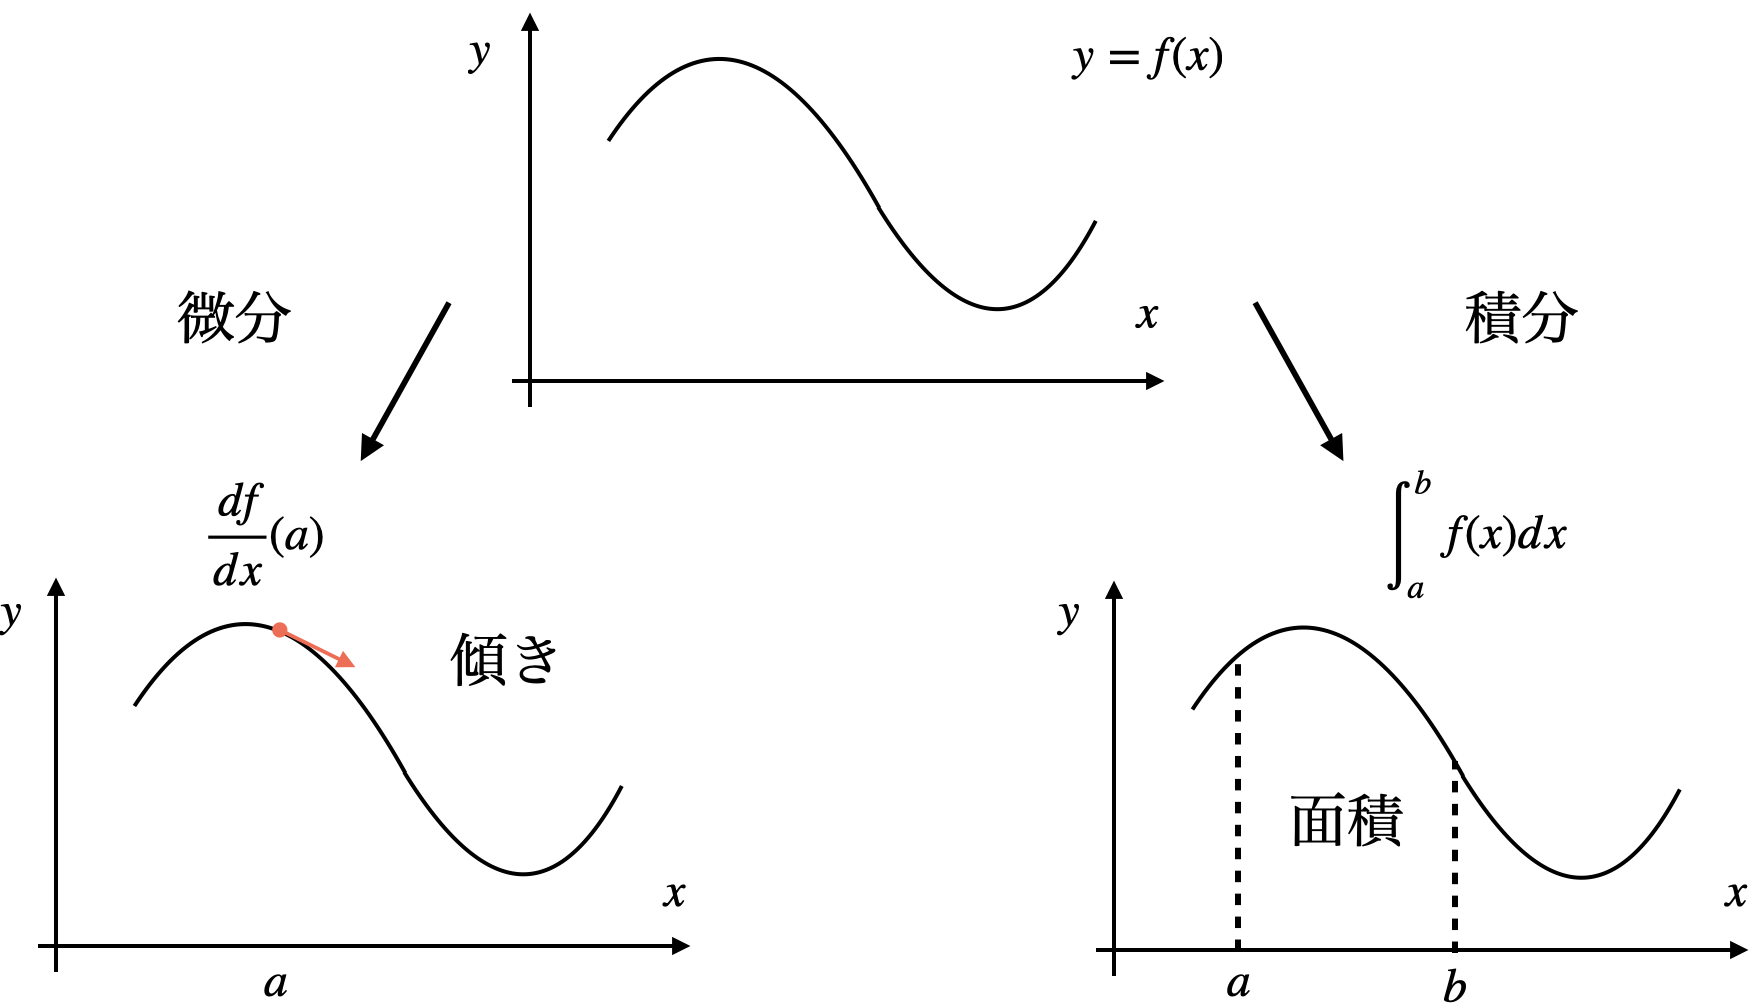
\includegraphics[width=100mm]{diff_int.png}
 \end{center}
\end{figure}

\end{frame}


%%%%%%%%%%%%%%%%%%%%%%%%%%%%%%%%%%%%%%%%%%%%%%%%%%%%%%%%%%%%%%%%%%%%%%%%%%%%%%%%%%%%%%%
%%%%%%%%%%%%%%%%%%%%%%%%%%%%%%%%%%%%%%%%%%%%%%%%%%%%%%%%%%%%%%%%%%%%%%%%%%%%%%%%%%%%%%%


\begin{frame}
\frametitle{微分}

微分: 最も値の大きい・小さいところを探す方法

 \begin{figure}[htbp]
 \begin{center} 
  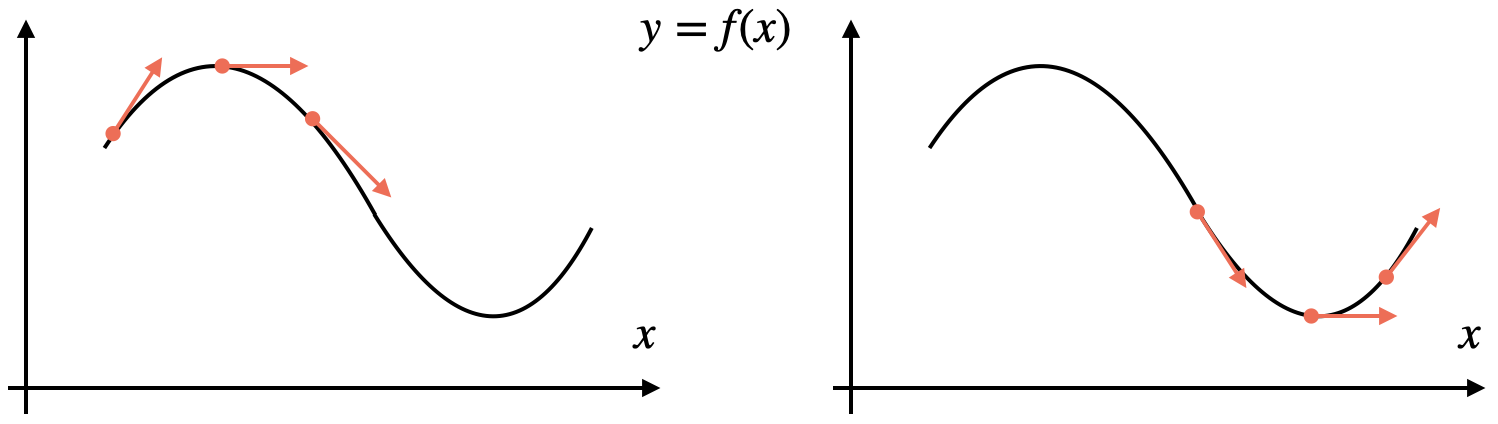
\includegraphics[width=100mm]{diff.png}
 \end{center}
\end{figure}


\begin{itemize}
\item 極大点の頂上の手前では坂は上がり, 先では下る. 
\item 極小点の底の手前では坂は下り, 先では上がる. 
\item 極大点, 極小点 $\Rightarrow$ 傾き0. 
\item グラフの傾き = 関数の値の変化率, 未来の判断材料. 
\end{itemize}

\end{frame}


%%%%%%%%%%%%%%%%%%%%%%%%%%%%%%%%%%%%%%%%%%%%%%%%%%%%%%%%%%%%%%%%%%%%%%%%%%%%%%%%%%%%%%%
%%%%%%%%%%%%%%%%%%%%%%%%%%%%%%%%%%%%%%%%%%%%%%%%%%%%%%%%%%%%%%%%%%%%%%%%%%%%%%%%%%%%%%%


\begin{frame}
\frametitle{応用}   

最適化問題: 適当な条件を満たす最適解を探す

\begin{itemize}
\item 等周問題: 周の長さが$l$の長方形の中で面積を最大にするものは? 
\item 面積$A(x)=x(l/2-x)$
\end{itemize}

 \begin{figure}[htbp]
 \begin{center} 
  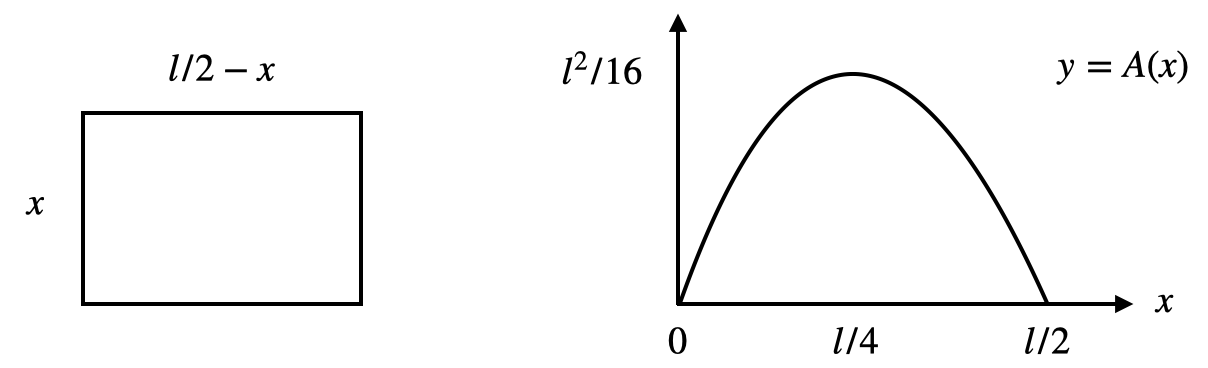
\includegraphics[width=100mm]{LecArea.png}
 \end{center}
\end{figure}

\end{frame}


%%%%%%%%%%%%%%%%%%%%%%%%%%%%%%%%%%%%%%%%%%%%%%%%%%%%%%%%%%%%%%%%%%%%%%%%%%%%%%%%%%%%%%%
%%%%%%%%%%%%%%%%%%%%%%%%%%%%%%%%%%%%%%%%%%%%%%%%%%%%%%%%%%%%%%%%%%%%%%%%%%%%%%%%%%%%%%%


\begin{frame}
\frametitle{積分}

積分: これまでの蓄積を計算する方法

 \begin{figure}[htbp]
 \begin{center} 
  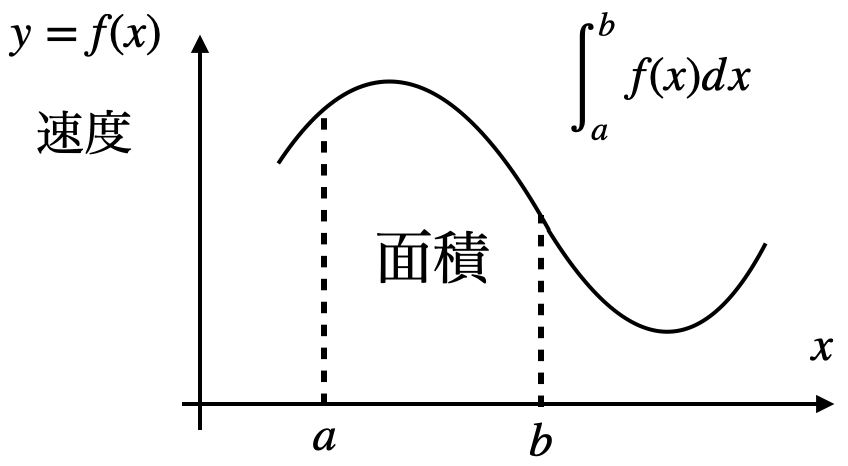
\includegraphics[width=60mm]{int_speed.png}
 \end{center}
\end{figure}


\begin{itemize}
\item 面積$\int_a^b f(x)dx$は時刻$a$から時刻$b$までに移動した距離. 
\item 平均速度 = 面積/時間. 
\item 面積 = 過去の蓄積, 過去の判断材料.
\end{itemize}

\end{frame}


%%%%%%%%%%%%%%%%%%%%%%%%%%%%%%%%%%%%%%%%%%%%%%%%%%%%%%%%%%%%%%%%%%%%%%%%%%%%%%%%%%%%%%%
%%%%%%%%%%%%%%%%%%%%%%%%%%%%%%%%%%%%%%%%%%%%%%%%%%%%%%%%%%%%%%%%%%%%%%%%%%%%%%%%%%%%%%%


\begin{frame}
\frametitle{積分}

時刻$a$から時刻$t$までに移動した距離は$F(t)=\int_a^tf(x)dx$で与えられた. 

 \begin{figure}[htbp]
 \begin{center} 
  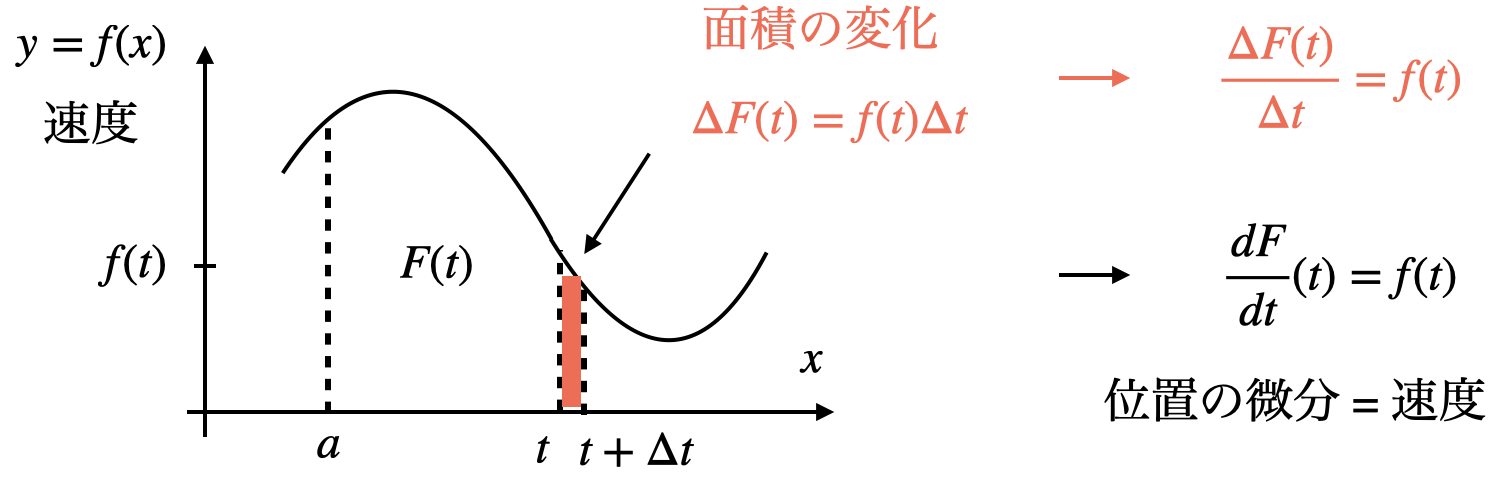
\includegraphics[width=100mm]{diff_pos=speed.png}
 \end{center}
\end{figure}


\begin{itemize}
\item 「速度」を積分すると「位置」(過去の蓄積). 
\item 「位置」を微分すると「速度」(現在の変化). 
\item  一般に, 微分と積分は逆操作. 
\end{itemize}

\end{frame}



%%%%%%%%%%%%%%%%%%%%%%%%%%%%%%%%%%%%%%%%%%%%%%%%%%%%%%%%%%%%%%%%%%%%%%%%%%%%%%%%%%%%%%%
%%%%%%%%%%%%%%%%%%%%%%%%%%%%%%%%%%%%%%%%%%%%%%%%%%%%%%%%%%%%%%%%%%%%%%%%%%%%%%%%%%%%%%%



\begin{frame}
\frametitle{微分・積分}

以上を簡単にまとめると

 \begin{figure}[htbp]
 \begin{center} 
  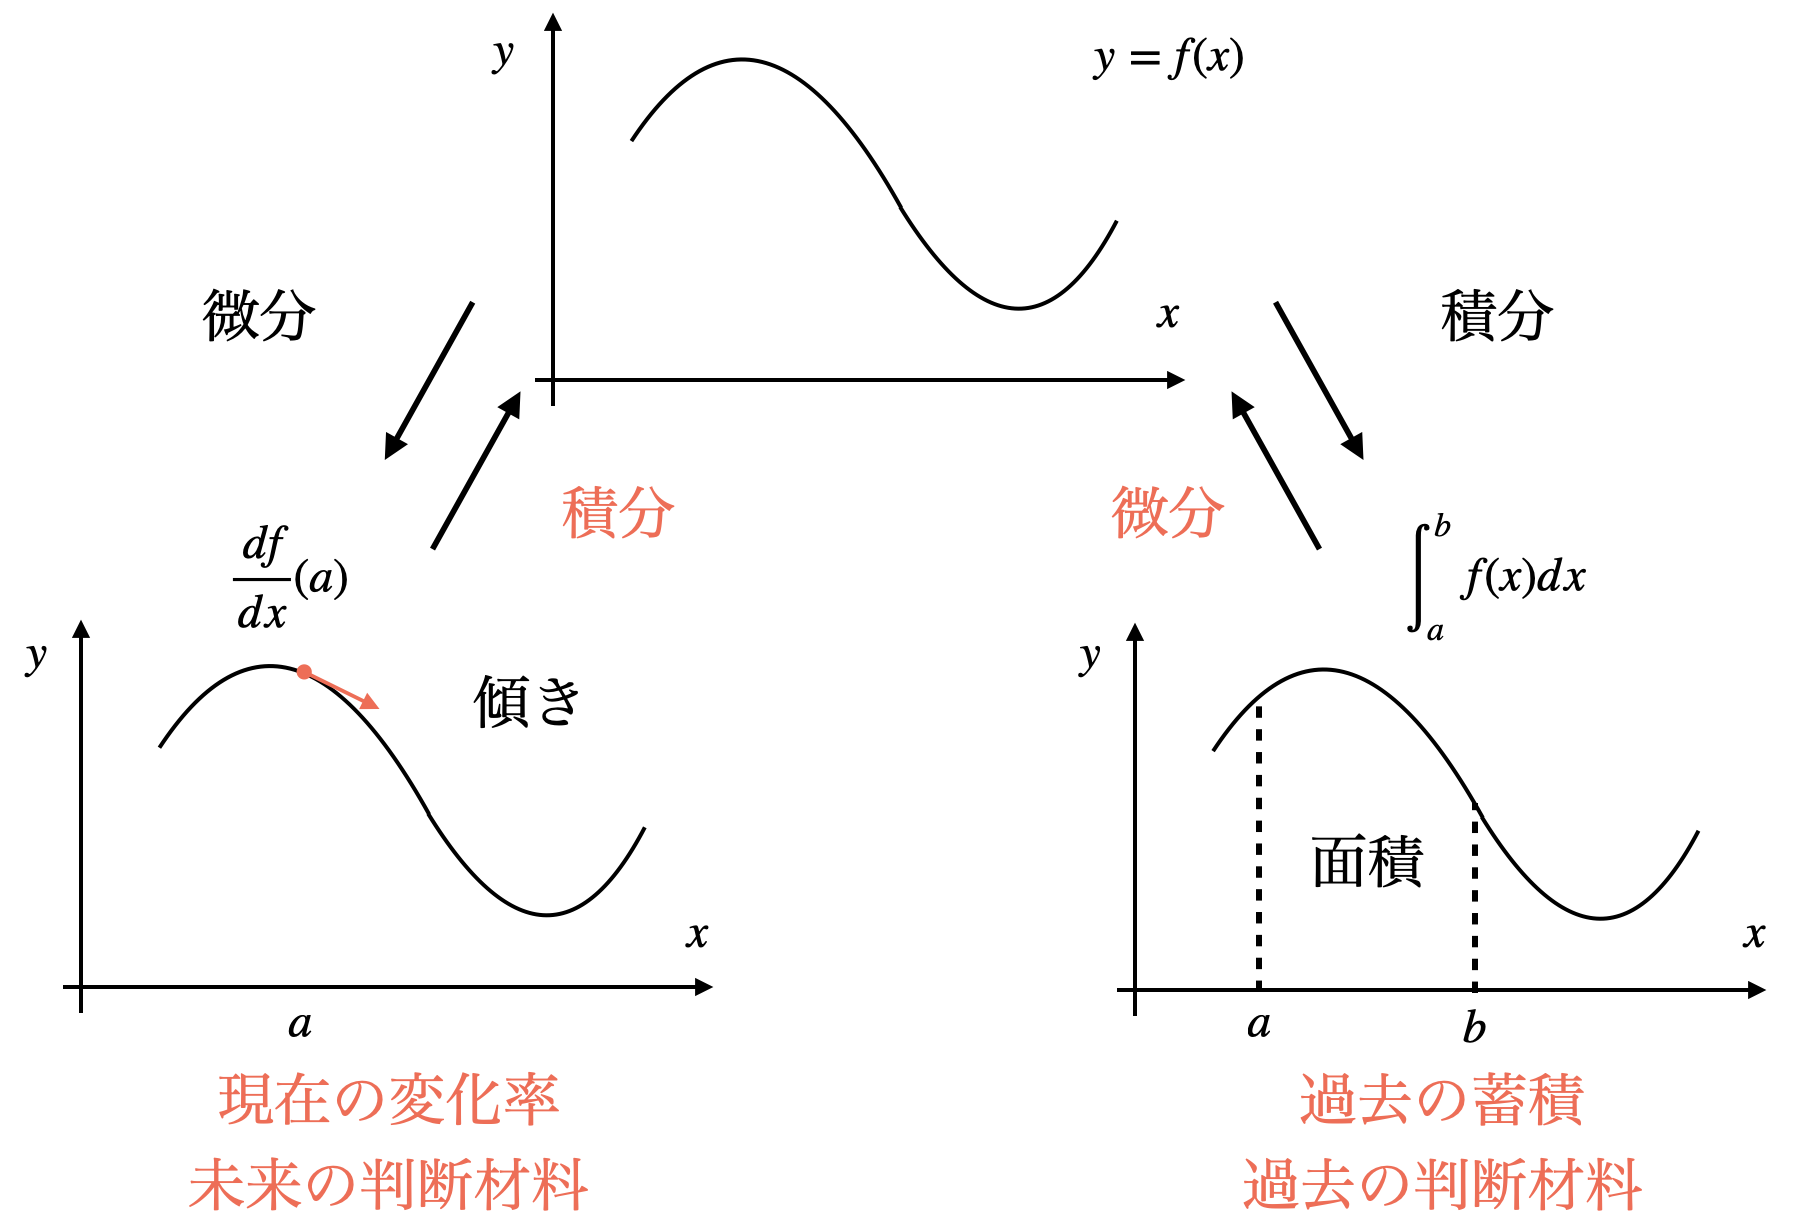
\includegraphics[width=100mm]{diff_int2.png}
 \end{center}
\end{figure}

\end{frame}






%%%%%%%%%%%%%%%%%%%%%%%%%%%%%%%%%%%%%%%%%%%%%%%%%%%%%%%%%%%%%%%%%%%%%%%%%%%%%%%%%%%%%%%
%%%%%%%%%%%%%%%%%%%%%%%%%%%%%%%%%%%%%%%%%%%%%%%%%%%%%%%%%%%%%%%%%%%%%%%%%%%%%%%%%%%%%%%
%%%%%%%%%%%%%%%%%%%%%%%%%%%%%%%%%%%%%%%%%%%%%%%%%%%%%%%%%%%%%%%%%%%%%%%%%%%%%%%%%%%%%%%
%%%%%%%%%%%%%%%%%%%%%%%%%%%%%%%%%%%%%%%%%%%%%%%%%%%%%%%%%%%%%%%%%%%%%%%%%%%%%%%%%%%%%%%


\section{集合論}

\begin{frame}
\frametitle{集合, 濃度}   

記号の準備も兼ねて, 集合論から始める. 

\begin{Def}
\begin{itemize}
\item 
対象(もの)の集まりを\underline{集合}という. 
対象となるものは, 数字, 記号, 文字列など色々考えられる. 
%ただし, その集まりに含まれるかどうか明確に識別できなければならない. 
\item
集合の構成要素を\underline{元}(要素)という. 
$a$が集合$A$の元であることを, $a \in A$と表す. 
$a$が$A$の元であるとき, $a$は$A$に含まれるということもある. 
$a \in A$の否定を$a \notin A$と書く. 
\item 
集合$A$の元の数を$|A|$で表し, $A$の\underline{濃度}(位数)と呼ぶ. 
集合$A$で
\begin{itemize}
\item $|A|=\infty$なるものは\underline{無限集合}, 
\item $|A| \ne \infty$なるものは\underline{有限集合}. 
\end{itemize}
\end{itemize}
\end{Def}


\end{frame}

%%%%%%%%%%%%%%%%%%%%%%%%%%%%%%%%%%%%%%%%%%%%%%%%%%%%%%%%%%%%%%%%%%%%%%%%%%%%%%%%%%%%%%%
%%%%%%%%%%%%%%%%%%%%%%%%%%%%%%%%%%%%%%%%%%%%%%%%%%%%%%%%%%%%%%%%%%%%%%%%%%%%%%%%%%%%%%%



\begin{frame}
\frametitle{集合}   

\begin{Ex}
\begin{enumerate}
%\item 整数$1, 3, 5, 7$を元に持つ集合$A=\{1,3,5,7\}$に関して, $1\in A$であるが$2 \notin A$である. 
%また$|A|=4$であるから, $A$は有限集合. 
\item $A=\{\text{りんご, みかん, バナナ}\}$とすれば, $\text{みかん} \in A$. 
\item 都道府県の集合
$$
A=\{\text{北海道, 青森県, 岩手県, 宮城県, \dots}\}
$$
は$|A|=47$. 
\item 
\begin{itemize}
\item $\N=\{1,2,3,\dots\}$:自然数, 
\item $\Z=\{ \dots, -2,-1,0,1,2,\dots \}$:整数, 
\item $\Q$:有理数(分数全体), $\R$:実数
\end{itemize}
これらは全て無限集合. 
\end{enumerate} 
\end{Ex}



\end{frame}



%%%%%%%%%%%%%%%%%%%%%%%%%%%%%%%%%%%%%%%%%%%%%%%%%%%%%%%%%%%%%%%%%%%%%%%%%%%%%%%%%%%%%%%
%%%%%%%%%%%%%%%%%%%%%%%%%%%%%%%%%%%%%%%%%%%%%%%%%%%%%%%%%%%%%%%%%%%%%%%%%%%%%%%%%%%%%%%


\begin{frame}
\frametitle{外延的記法} 

集合を定義するには, その集合に含まれる元を指定すれば良い. \\
\ \\

\underline{外延的記法}: その集合が持つ元を全て列挙する直接的な方法. 例えば
$$
\{1,2,3,4\}, \ \{\text{子豚, 狸, 狐, 猫}\}, \ \{1,3,5,7,9,11,\dots\}. 
$$
最後の集合は奇数全体の集合を意図したものだが, 「$\dots$」に何が並ぶのかが明確でないと誤解を招く恐れがある. 


\begin{Ex}
自然数の集合
$$
\N=\{1,2,3,4,5,\dots\}. 
$$
整数の集合
$$
\Z=\{\dots, -2,-1,0,1,2,\dots\}. 
$$
\end{Ex}

\end{frame}

%%%%%%%%%%%%%%%%%%%%%%%%%%%%%%%%%%%%%%%%%%%%%%%%%%%%%%%%%%%%%%%%%%%%%%%%%%%%%%%%%%%%%%%
%%%%%%%%%%%%%%%%%%%%%%%%%%%%%%%%%%%%%%%%%%%%%%%%%%%%%%%%%%%%%%%%%%%%%%%%%%%%%%%%%%%%%%%


\begin{frame}
\frametitle{内包的記法}   

 \underline{内包的記法}: 集合に含まれる元の条件を明示する方法. 
「命題$P$が真となる$x \in X$全体の集合」を
$$
\{ x \in X \ | \ P\}
$$
と書く. 
ここで$X$は変数$x$が動く範囲の集合である.  
例えば
$$
\{n \in \Z \ | \ -1.4 \le n \le 3\}
$$
は「整数$n$であって$-1.4 \le n \le 3$が成立するもの全体の集合」と読む. 
外延的方法を用いれば, これは
$$
\{-1,0,1,2,3\}
$$
とも表せる. 

\end{frame}



%%%%%%%%%%%%%%%%%%%%%%%%%%%%%%%%%%%%%%%%%%%%%%%%%%%%%%%%%%%%%%%%%%%%%%%%%%%%%%%%%%%%%%%
%%%%%%%%%%%%%%%%%%%%%%%%%%%%%%%%%%%%%%%%%%%%%%%%%%%%%%%%%%%%%%%%%%%%%%%%%%%%%%%%%%%%%%%


\begin{frame}
\frametitle{外延的方法 vs 内包的記法}   

\begin{Ex}
実数$a<b$に対して, $a,b$を端点とする閉区間, 開区間が
\begin{align*}
[a,b] = \{x \in \R \ | \ a \le x \le b \}, \ \ (a,b) &=\{x \in \R \ | \ a < x < b \} 
\end{align*}
で定義される. 
同様に半開区間
\begin{align*}
(a,b] = \{x \in \R \ | \ a < x \le b \}, \ \ [a,b) &=\{x \in \R \ | \ a \le x < b \}
\end{align*}
が定義される. 
これらは外延的方法では記述できない無限集合である. 
\end{Ex}

2つの黒丸に挟まれた区間が閉空間, 2つの白丸に挟まれた区間が開空間: 
 \begin{figure}[htbp]
 \begin{center} 
  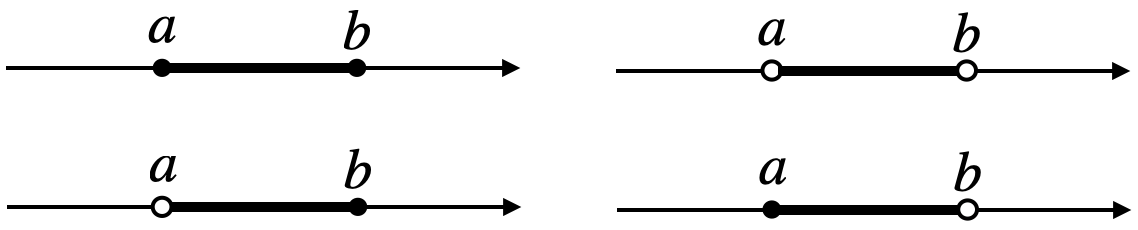
\includegraphics[width=80mm]{interval.png}
 \end{center}
\end{figure}

\end{frame}




%%%%%%%%%%%%%%%%%%%%%%%%%%%%%%%%%%%%%%%%%%%%%%%%%%%%%%%%%%%%%%%%%%%%%%%%%%%%%%%%%%%%%%%
%%%%%%%%%%%%%%%%%%%%%%%%%%%%%%%%%%%%%%%%%%%%%%%%%%%%%%%%%%%%%%%%%%%%%%%%%%%%%%%%%%%%%%%


\begin{frame}
\frametitle{直積集合}   

\begin{Def}[直積集合]
$A, B$を集合とする. 
$a \in A$と$b \in B$を並べた$(a,b)$を\underline{順序対}という. 
順序対全体のなす集合を$A$と$B$の\underline{直積集合}といい, $A \times B$と書く. 
$$
A \times B = \{(a,b) \ | \ a \in A, \ b \in B\}. 
$$
\end{Def}

$A=\{a,b\}, B=\{c,d\}$とすれば
\begin{align}
A\times B &= \{(x,y) \ | \ x \in A, \ y \in B \} \notag \\
&=\{(a,c), (a,d), (b,c), (b,d)\}.  \notag
\end{align}

同様に3つの集合$A,B,C$の直積集合$A \times B \times C$や, $n$個の集合$A_1,\dots,A_n$の直積集合
$$
A_1 \times \dots \times A_n
$$
が定義される. 



\end{frame}



%%%%%%%%%%%%%%%%%%%%%%%%%%%%%%%%%%%%%%%%%%%%%%%%%%%%%%%%%%%%%%%%%%%%%%%%%%%%%%%%%%%%%%%
%%%%%%%%%%%%%%%%%%%%%%%%%%%%%%%%%%%%%%%%%%%%%%%%%%%%%%%%%%%%%%%%%%%%%%%%%%%%%%%%%%%%%%%



\begin{frame}
\frametitle{$n$次元座標空間$\R^n$}   


\begin{Ex}
\begin{itemize}
\item 実数全体の集合$\R$は実直線$\R^1$と同一視することができた. 
\item 実平面
$$
\R^2=\R \times \R=\{(x,y) \ | \ x \in \R, \ y \in \R\}
$$
\item $3$次元座標空間
$$
\R^3=\R \times \R \times \R=\{(x,y,z) \ | \ x \in \R, \ y \in \R \ z\in \R\}
$$
\item 一般に, $\R^n$は$n$次元座標空間, もしくは$n$次元ユークリッド空間と呼ばれる. 
\end{itemize}
\end{Ex}

この講義では主に$\R, \R^2,\R^3$を扱う. 

\end{frame}

%%%%%%%%%%%%%%%%%%%%%%%%%%%%%%%%%%%%%%%%%%%%%%%%%%%%%%%%%%%%%%%%%%%%%%%%%%%%%%%%%%%%%%%
%%%%%%%%%%%%%%%%%%%%%%%%%%%%%%%%%%%%%%%%%%%%%%%%%%%%%%%%%%%%%%%%%%%%%%%%%%%%%%%%%%%%%%%


%\begin{frame}
%\frametitle{直積集合}   
%
%\begin{Ex}
%必ずしも同じような集合の直積を取る必要はない. 
%例えば
%$$
%A=\{\text{りんご, みかん, バナナ}\}, \ \ \ B=\{-3,7\}
%$$
%とすれば, $A\times B$は
%\begin{align}
%&\{(\text{りんご},-3), (\text{みかん},-3), (\text{バナナ},-3), \notag \\
%& \ \ \ (\text{りんご},7),  (\text{みかん},7), (\text{バナナ},7)\} \notag 
%\end{align}
%なる6つの元を持つ集合である. 
%\end{Ex}
%
%
%\end{frame}



%%%%%%%%%%%%%%%%%%%%%%%%%%%%%%%%%%%%%%%%%%%%%%%%%%%%%%%%%%%%%%%%%%%%%%%%%%%%%%%%%%%%%%%
%%%%%%%%%%%%%%%%%%%%%%%%%%%%%%%%%%%%%%%%%%%%%%%%%%%%%%%%%%%%%%%%%%%%%%%%%%%%%%%%%%%%%%%


\begin{frame}
\frametitle{包含関係}   


複数の集合があるとき, それらの間の関係を考えることは自然である.  
最も基本的なものが\underline{包含関係}である.

\begin{Def}[部分集合]
$A, B$を集合とする.
\begin{enumerate}
\item 任意の$A$の元が$B$の元でもあるとき, $A$は$B$の\underline{部分集合}であるといい, $A \subset B$と書く.  
%すなわち, $A \subset B$であるとは, $x \in A \Rightarrow x \in B$が成立することである. 
$A \subset B$でないとき, $A \not\subset B$と書く.
\item $A \subset B$かつ$B \subset A$のとき, $A$と$B$は\underline{(集合として)等しい}といい, $A=B$と書く. 
\item $A \subset B$かつ$A \ne B$ のとき, $A$は$B$の\underline{真部分集合}であるといい, $A \subsetneq B$とかく.
\end{enumerate} 
\end{Def}


\end{frame}


%%%%%%%%%%%%%%%%%%%%%%%%%%%%%%%%%%%%%%%%%%%%%%%%%%%%%%%%%%%%%%%%%%%%%%%%%%%%%%%%%%%%%%%
%%%%%%%%%%%%%%%%%%%%%%%%%%%%%%%%%%%%%%%%%%%%%%%%%%%%%%%%%%%%%%%%%%%%%%%%%%%%%%%%%%%%%%%


\begin{frame}
\frametitle{包含関係}   

人間の集合を$\{\text{人間}\}$と略記したりする. 
これは人間1人からなる集合ではない. 

\begin{Ex}
\begin{enumerate}
\item $\{\text{人間}\} \subset \{\text{哺乳類}\}$, $\{\text{犬}\} \subset \{\text{哺乳類}\}$
\item $\N \subset \Z \subset \Q \subset  \R$
\item 実数$a<b$に対して, $(a,b) \subsetneq [a,b]$である. 
一方で, $(a,b]$と$[a,b)$の間には包含関係はない. 
\end{enumerate} 
\end{Ex}


 \begin{figure}[htbp]
 \begin{center} 
  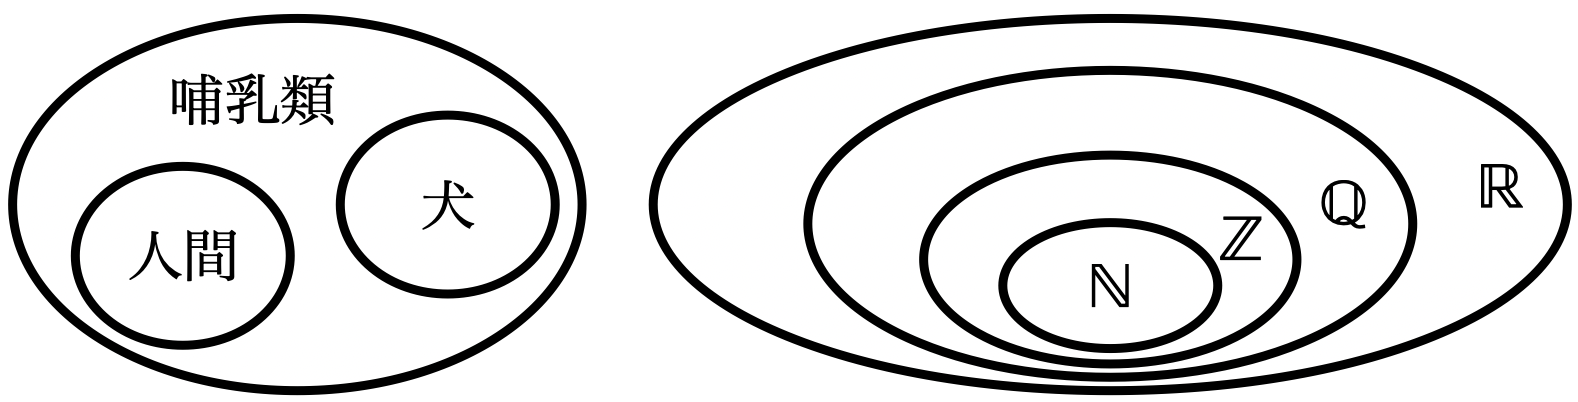
\includegraphics[width=100mm]{subsets.png}
 \end{center}
\end{figure}

\end{frame}



%%%%%%%%%%%%%%%%%%%%%%%%%%%%%%%%%%%%%%%%%%%%%%%%%%%%%%%%%%%%%%%%%%%%%%%%%%%%%%%%%%%%%%%
%%%%%%%%%%%%%%%%%%%%%%%%%%%%%%%%%%%%%%%%%%%%%%%%%%%%%%%%%%%%%%%%%%%%%%%%%%%%%%%%%%%%%%%


%\begin{frame}
%\frametitle{空集合}   
%
%
%\begin{Def}[空集合]
%元を1つも含まない集合を\underline{空集合}といい, $\emptyset$とかく. 
%外延的方法を用いれば
%$$
%\emptyset=\{\}
%$$
%である. 
%どんな集合$A$に対しても, $\emptyset \subset A$が成立する.  
%%これは約束と思っても良いし, 次のようにして導くことも できる. 空集合は元を一つも含まないのだから, x ∈ \UTF{2205} は任意の x に対して偽である. 
%%そ こで,「x∈\UTF{2205}⇒x∈A」は真である. よって,\UTF{2205}⊂Aとなる.
%\end{Def}
%
%
%\begin{Ex}
%集合$A=\{1,2,3\}$の部分集合を全て列挙すると
%$$
%\emptyset, \{1\},\{2\},\{3\}, \{1,2\},\{2,3\},\{3,1\},\{1,2,3\} 
%$$
%の8つである. 
%\end{Ex}
%
%
%
%\end{frame}




%%%%%%%%%%%%%%%%%%%%%%%%%%%%%%%%%%%%%%%%%%%%%%%%%%%%%%%%%%%%%%%%%%%%%%%%%%%%%%%%%%%%%%%
%%%%%%%%%%%%%%%%%%%%%%%%%%%%%%%%%%%%%%%%%%%%%%%%%%%%%%%%%%%%%%%%%%%%%%%%%%%%%%%%%%%%%%%

\section{写像}

\begin{frame}
\frametitle{写像}

\begin{Def} \label{写像定義}
\begin{itemize}
\item 集合$X$の各元に対して, 集合$Y$の元を唯一つ定める対応のことを写像と呼び, $f:X \rightarrow Y$と表す. 
$X$を\underline{定義域}, $Y$を\underline{値域}という. 
\item 写像$f:X\rightarrow Y$によって$x \in X$が$y\in Y$に対応するとき, $y$を$f$による$x$の\underline{像}といい, $y=f(x)$と書く. 
この対応を次のように書く. \vspace{-1mm}
$$
f:X \longrightarrow Y, \ \ \ x \mapsto y. 
$$
\end{itemize}
\end{Def}

\vspace{-1mm}

 \begin{figure}[htbp]
 \begin{center} 
  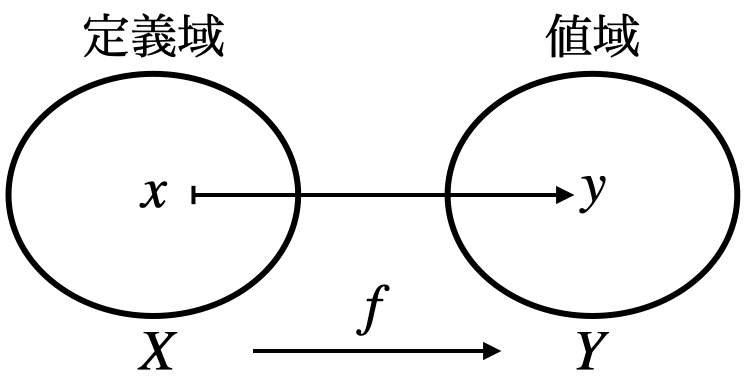
\includegraphics[width=50mm]{map.png}
 \end{center}
\end{figure}

\vspace{-1mm}

\end{frame}


%%%%%%%%%%%%%%%%%%%%%%%%%%%%%%%%%%%%%%%%%%%%%%%%%%%%%%%%%%%%%%%%%%%%%%%%%%%%%%%%%%%%%%%
%%%%%%%%%%%%%%%%%%%%%%%%%%%%%%%%%%%%%%%%%%%%%%%%%%%%%%%%%%%%%%%%%%%%%%%%%%%%%%%%%%%%%%%




\begin{frame}
\frametitle{写像}


\begin{Ex}
\begin{enumerate}
\item $f:\{\text{人間}\} \longrightarrow \Z, \ \ \ A \mapsto \text{$A$の年齢}$
\item $g:\{\text{犬}\} \longrightarrow \R, \ \ \ A \mapsto \text{$A$の身長}$
\item $h:\{\text{猫}\} \longrightarrow \{\text{猫}\}, \ \ \ A \mapsto \text{$A$の母猫}$
\item $i:\{\text{日本の大学}\} \longrightarrow \N, \ \ \ \text{$A$大学} \mapsto \text{$A$大学の学生数}$
\item $j:\{\text{日本の大学}\} \longrightarrow \{\text{都道府県}\}, \ \ \ \text{$A$大学} \mapsto \text{$A$大学の所在地}$
\end{enumerate}
一方で, 人間$A$と$A$の友人の対応は写像ではない. 
$A$の友人が1人とは限らないからである. 
\end{Ex}


\end{frame}



%%%%%%%%%%%%%%%%%%%%%%%%%%%%%%%%%%%%%%%%%%%%%%%%%%%%%%%%%%%%%%%%%%%%%%%%%%%%%%%%%%%%%%%
%%%%%%%%%%%%%%%%%%%%%%%%%%%%%%%%%%%%%%%%%%%%%%%%%%%%%%%%%%%%%%%%%%%%%%%%%%%%%%%%%%%%%%%


\begin{frame}
\frametitle{像}


\begin{Def}
写像$f:X\rightarrow Y$の\underline{像}を
$$
\Imag f = \{ f(x) \ | \ x \in X\}
$$
で定義する. 
つまり$x$が$X$の全ての元を動くとき, $x$の像$f(x)$全体のなす$Y$の部分集合のことである. 
\end{Def}


 \begin{figure}[htbp]
 \begin{center} 
  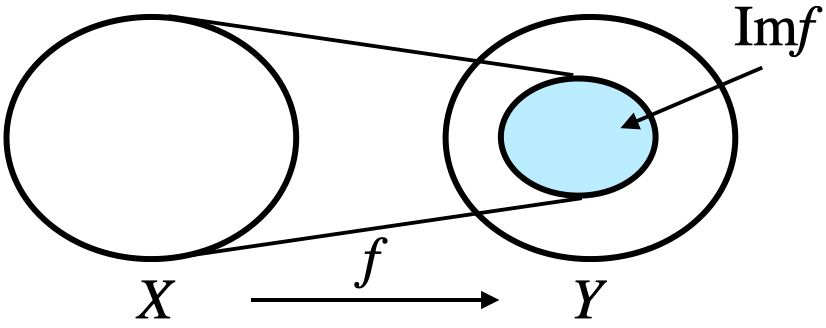
\includegraphics[width=50mm]{imf.png}
 \end{center}
\end{figure}


\end{frame}

%%%%%%%%%%%%%%%%%%%%%%%%%%%%%%%%%%%%%%%%%%%%%%%%%%%%%%%%%%%%%%%%%%%%%%%%%%%%%%%%%%%%%%%
%%%%%%%%%%%%%%%%%%%%%%%%%%%%%%%%%%%%%%%%%%%%%%%%%%%%%%%%%%%%%%%%%%%%%%%%%%%%%%%%%%%%%%%


\begin{frame}
\frametitle{全射, 単射}


\begin{Def}$f:X\rightarrow Y$を写像とする. 
\begin{enumerate}
\item $f$が\underline{全射}であるとは$\Imag f = Y$が成立すること. 
つまり「どの$y \in Y$に対しても$x \in X$が存在して$y=f(x)$」. 
\item $f$が\underline{単射}であるとは「$x_1\ne x_2$ならば$f(x_1)\ne f(x_2)$」が成立すること. 
同値な対偶条件は「$f(x_1)= f(x_2)$ならば$x_1= x_2$」.  
\item $f$が\underline{全単射}であるとは, 全射かつ単射であること. 
\end{enumerate}
\end{Def}



\end{frame}

%%%%%%%%%%%%%%%%%%%%%%%%%%%%%%%%%%%%%%%%%%%%%%%%%%%%%%%%%%%%%%%%%%%%%%%%%%%%%%%%%%%%%%%
%%%%%%%%%%%%%%%%%%%%%%%%%%%%%%%%%%%%%%%%%%%%%%%%%%%%%%%%%%%%%%%%%%%%%%%%%%%%%%%%%%%%%%%


\begin{frame}
\frametitle{全射, 単射}

\begin{Ex}
\begin{enumerate}
\item $f:\R \rightarrow \R, x \mapsto x^2(x-1)$は(全射だが)単射ではない. 
\item $g:\R \rightarrow \R, x \mapsto x^2$は全射でも単射でもない. $\Imag g=\R_{\ge 0}$. 
\item $h:\R \rightarrow \R, x \mapsto x^3$は全単射である. 
\end{enumerate}
\end{Ex}


\begin{Prob}
次の写像は全射か? 単射か? 
\begin{enumerate}
\item $f:\Z \rightarrow \Z, x \mapsto x^2(x-1)$.  
\item $g:\Z \rightarrow \Z, x \mapsto x^2$.
\item $h:\Z \rightarrow \Z, x \mapsto x^3$. 
\end{enumerate}
\end{Prob}



\end{frame}



%%%%%%%%%%%%%%%%%%%%%%%%%%%%%%%%%%%%%%%%%%%%%%%%%%%%%%%%%%%%%%%%%%%%%%%%%%%%%%%%%%%%%%%
%%%%%%%%%%%%%%%%%%%%%%%%%%%%%%%%%%%%%%%%%%%%%%%%%%%%%%%%%%%%%%%%%%%%%%%%%%%%%%%%%%%%%%%


\begin{frame}
\frametitle{全射, 単射, 恒等写像}

\begin{Ex}
次の写像を考える: 
\begin{align*}
f: & \{\text{日本の大学}\} \longrightarrow \N, \ \ \ \text{$A$大学} \mapsto \text{$A$大学の学生数} \\
g:& \{\text{日本の大学}\} \longrightarrow \{\text{都道府県}\}, \ \ \ \text{$A$大学} \mapsto \text{$A$大学の所在地}
\end{align*}
写像$f$は全射ではない(単射であろうか?). 写像$g$は全射だが, 単射ではない. 
\end{Ex}


\begin{Ex}
何もしない写像$\id :X \rightarrow X, x \mapsto x$を\underline{恒等写像}という. 
恒等写像は全単射である. 
\end{Ex}


\end{frame}



%%%%%%%%%%%%%%%%%%%%%%%%%%%%%%%%%%%%%%%%%%%%%%%%%%%%%%%%%%%%%%%%%%%%%%%%%%%%%%%%%%%%%%%
%%%%%%%%%%%%%%%%%%%%%%%%%%%%%%%%%%%%%%%%%%%%%%%%%%%%%%%%%%%%%%%%%%%%%%%%%%%%%%%%%%%%%%%


\begin{frame}
\frametitle{全射, 単射, 恒等写像}

\begin{Prob}
次の写像は全射か? 単射か? 
\begin{enumerate}
\item 慶應義塾大学の学生に対して, 学籍番号を対応させる写像
$$
f:\{ \text{慶応義塾生}\} \longrightarrow \Z^8
$$
\item 値域を学籍番号となる番号に限ったらどうであろうか? 
$$
g:\{ \text{慶応義塾生}\} \longrightarrow \{ \text{学籍番号}\} \subset \Z^8
$$
\end{enumerate}
\end{Prob}

\end{frame}




%%%%%%%%%%%%%%%%%%%%%%%%%%%%%%%%%%%%%%%%%%%%%%%%%%%%%%%%%%%%%%%%%%%%%%%%%%%%%%%%%%%%%%%
%%%%%%%%%%%%%%%%%%%%%%%%%%%%%%%%%%%%%%%%%%%%%%%%%%%%%%%%%%%%%%%%%%%%%%%%%%%%%%%%%%%%%%%


\begin{frame}
\frametitle{合成写像}

\begin{Def}
写像$f:X \rightarrow Y, g:Y\rightarrow Z$に対して, \underline{合成写像}$g\circ f: X\rightarrow Z$が
$$
g\circ f(x)=g(f(x))
$$
で定義される. つまり$x \in X$に対して$f(x) \in Y$が定まり, さらに$f(x) \in Y$に対して$g(f(x)) \in Z$が定まる. 
図示すれば次のようになる. 
$$
\xymatrix{
X \ar[r]^{f} \ar@/_15pt/[rr]_{g\circ f} &  Y \ar[r]^{g}& Z
}
$$
\end{Def}

$f:X \rightarrow Y, g:Y\rightarrow Z$の合成写像の表記「$g\circ f$」において$f,g$の順序に注意する. 
これは合成写像が$g(f(x))$で定義されていることから理解できる. 


\end{frame}


%%%%%%%%%%%%%%%%%%%%%%%%%%%%%%%%%%%%%%%%%%%%%%%%%%%%%%%%%%%%%%%%%%%%%%%%%%%%%%%%%%%%%%%
%%%%%%%%%%%%%%%%%%%%%%%%%%%%%%%%%%%%%%%%%%%%%%%%%%%%%%%%%%%%%%%%%%%%%%%%%%%%%%%%%%%%%%%


\begin{frame}
\frametitle{逆写像}


\begin{Thm}
写像$f:X\rightarrow Y$が全単射であれば, 写像$g:Y\rightarrow X$が存在して, 
$$
g\circ f = \id, \ \ \ f \circ g = \id
$$
が成立する. 
この$g$を$f$の\underline{逆写像}といい, $f^{-1}$と書く. 
\end{Thm}

実際, 任意の$y \in Y$に対して, $x \in X$で$f(x)=y$なるものが唯一つ存在するので, $g(y)=x$と定義すれば良い. 
%これを$f^{-1}(y)=x$と書くということである. 
\vspace{-2mm}

 \begin{figure}[htbp]
 \begin{center} 
  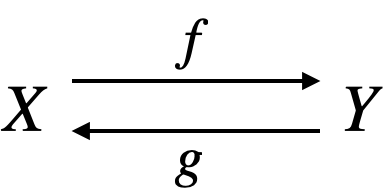
\includegraphics[width=25mm]{inverse.png}
 \end{center}
\end{figure}

\end{frame}




%%%%%%%%%%%%%%%%%%%%%%%%%%%%%%%%%%%%%%%%%%%%%%%%%%%%%%%%%%%%%%%%%%%%%%%%%%%%%%%%%%%%%%%
%%%%%%%%%%%%%%%%%%%%%%%%%%%%%%%%%%%%%%%%%%%%%%%%%%%%%%%%%%%%%%%%%%%%%%%%%%%%%%%%%%%%%%%


\begin{frame}
\frametitle{逆写像}


\begin{Ex}
先ほど議論した, 慶応義塾生に学籍番号を対応させる写像は全単射であった. 
$$
g:\{ \text{慶応義塾生}\} \longrightarrow \{ \text{学籍番号}\} \subset \Z^8
$$
逆写像は, 学籍番号から学生を特定することに対応する. 
\end{Ex}


\end{frame}



%%%%%%%%%%%%%%%%%%%%%%%%%%%%%%%%%%%%%%%%%%%%%%%%%%%%%%%%%%%%%%%%%%%%%%%%%%%%%%%%%%%%%%%
%%%%%%%%%%%%%%%%%%%%%%%%%%%%%%%%%%%%%%%%%%%%%%%%%%%%%%%%%%%%%%%%%%%%%%%%%%%%%%%%%%%%%%%


\begin{frame}
\frametitle{逆写像}



\begin{Ex}
写像$f:\R \rightarrow \R$, $x \mapsto 2x-4$は全単射である. 
$f$の逆写像は$g:\R \rightarrow \R$, $y \mapsto \frac{1}{2}y+2$で与えられる. 
実際, 
\begin{align*}
x & \ \ \mapsto \ \ 2x-4 \ \ \mapsto \ \ \frac{1}{2}(2x-4)+2=x \\
y & \ \ \mapsto \ \ \frac{1}{2}y+2 \ \ \mapsto \ \ 2(\frac{1}{2}y+2)-4 = y. 
\end{align*}
なので$g(f(x))=x$かつ$f(g(y))=y$. 
\end{Ex}
$f(x)=2x-4$の逆写像は, 方程式$y=2x-4$を$x$に関して解くことで求まる. 


\end{frame}



%%%%%%%%%%%%%%%%%%%%%%%%%%%%%%%%%%%%%%%%%%%%%%%%%%%%%%%%%%%%%%%%%%%%%%%%%%%%%%%%%%%%%%%
%%%%%%%%%%%%%%%%%%%%%%%%%%%%%%%%%%%%%%%%%%%%%%%%%%%%%%%%%%%%%%%%%%%%%%%%%%%%%%%%%%%%%%%





\section{今日のまとめ}
\begin{frame}
\frametitle{まとめ}   



\begin{enumerate}
\item 微分・積分の概要
\item 集合 (濃度, 外延的記法, 内包的記法, 直積集合, 包含関係)
\item 写像 (全射, 単射, 恒等写像, 合成写像, 逆写像)
\end{enumerate}


\end{frame}


\end{document}